\documentclass[twocolumn,floatfix,nofootinbib,aps]{revtex4-1}
\usepackage[utf8]{inputenc}

\usepackage{amsmath}    % need for subequations
\usepackage{amssymb}    % for symbols
\usepackage{graphicx}   % need for figures
\usepackage{verbatim}   % useful for program listings
\usepackage{color}      % use if color is used in text
\usepackage{subfigure}  % use for side-by-side figures
\usepackage{hyperref}   % use for hypertext links, including those to external documents and URLs
%\usepackage[capitalise]{cleveref}   % use for referencing figures/equations
\begin{document}

\title{Statistical Modeling of Conformational Dynamics \\ {\normalsize Second Year Progress Report}}
\author{Robert T. McGibbon} 
\affiliation{
 Department of Chemistry, Stanford University, Stanford, California 94305, USA
}
\date{August 27, 2013}

\begin{abstract}
Statistical modeling of long timescale dynamics with Markov state models (MSMs) has been shown to be an effective strategy for building quantitative and qualitative insight into long-time scale biomolecular conformational dynamics. Nonetheless, significant difficulties remain in the construction of MSMs, especially with regard to statistical and practical questions like overfitting and model selection. In this progress report, I introduce the topic, paying special attention to methodological issues and trade offs involved in the construction of the state space. I review recent work (McGibbon, R.T.; Pande, V. S.; \emph{J. Chem. Theory Comput.} 2013, 9, 2900) using large-margin machine learning to more optimally construct the MSM state space to yield an accurate kinetic model without relying upon the claim that geometric similarity provides an adequate basis for the kinetic partitioning of phase space. Finally, I introduce directions for future research in the field that I hope to contribute to over the course of my Ph.D.
\end{abstract}

\maketitle

\section{Introduction}
Protein dynamics are an essential aspect of biomolecular function. These dynamics span a wide range of length scales, timescales and complexity, including folding and aggregation, the conformational change between functional native sub-states, ligand binding, and allostery \cite{Dobson2003Protein, Kim2008Real, Austin1975Dynamics, Bahar2007Intrinsic}. Whereas classical experimental probes have often been interpreted in two-state frameworks, ensemble measurements with increasingly high temporal resolution as well as sensitive single molecule probes have uncovered a vast array of complex kinetics occurring via various pathways and with multiple intermediates \cite{Cosa2006Evidence, Zhang2011Direct}. But atomic-resolution structural characterization of these dynamics is often a Herculean challenge, particularly in dynamical settings -- as molecular probes like F\"{o}rster resonance energy transfer, small-angle x-ray scattering, and nuclear magnetic resonance techniques measure complex projections of the intrinsic structure, generally reporting simultaneously on many degrees of freedom\cite{Mertens2010Structural, Tzeng2011Protein}.

Computer simulations can complement experiments by providing atomic-resolution insight into the structural dynamics of biological molecules. With advances at the algorithmic, hardware, and software levels, modern molecular simulation paradigms, incorporating specialized or accelerated hardware, often in combination with highly parallel distributed computing frameworks, are capable of generating extensive simulation data sets\cite{Eastman2013OpenMM, Shirts2000Screen, Shaw2009Millisecond, Hess2008PLINCS}. In fact, the minimally-biased kinetic analysis of such simulations is often a central bottleneck and presents a major challenge to the field. The analysis paradigms often entail the construction of lower resolution models parametrized from the high resolution simulation data set which capture the essential features in an interpretable framework\cite{Freddolino2010Challenges, Lane2013Milliseconds}. For example, by projecting the data down onto one or two degrees of freedom we create a simpler model for the system, such as one characterized by diffusion along a single reaction coordinate\cite{Best2010Coordinate}.

Markov state models (MSMs) are one approach for analyzing MD data sets and driving further MD simulations that are able to smoothly move between high and low-resolution models\cite{Pande2010Everything, Beauchamp2012Simple, Prinz2011Markov, Bowman2013Quantitative}. Such detailed models maintain quantitative agreement with the underlying simulation data, while low-resolution models capture the salient features of the potential energy landscape, sacrificing some degree of model complexity. In an MSM, the dynamics are modeled as a memory-less jump process between a discrete set of conformational states. The two key quantities which define the MSM are thus the state definitions, an indicator function basis over phase space, and the pairwise transition probabilities or transition rates, which parametrize the kinetics. Via these models, parametrized directly from simulations with atomic-resolutions, we hope to synthesize many short simulations into a single model and directly connect to experimental biophysical measurements in a predictive and falsifiable manner.

Nonetheless, many challenges remain in the construction of Markov state models, especially with regard to statistical and practical questions like optimal model selection, integration with simulation engines in an ``active learning'' framework, further protocol automation, and development of richer model classes. In this report, I will introduce a set of methodological improvements for Markov state model construction developed by \textcite{McGibbon2013Learning}, and briefly sketch future directions for the field and for my own research. 

\section{Learning Distance Metrics: KDML}

Biomolecular systems are characterized by complex and high-dimensional conformational state spaces, with the possibility for multiple independent slow degrees of freedom as well as a large manifold of quickly-equilibrating degrees of freedom, such as C-H bond vibrations\footnote{Although CH bond vibrations are often constrained during simulations to permit longer time steps, this only further illustrates the points that not all degrees of freedom are essential for long-time scale dynamics.} or often side-chain orientations.

A significant challenge in the automated construction of Markov state models is the construction of the states. Although classical Hamiltonian dynamics form a continuous-time Markov chain in $\mathbb{R}^{6N}$\cite{vanKampen:2007ug}, the Markov property does not hold after the projecting the dynamics onto a basis of discrete indicator functions. In particular, when states contain within them free energy barriers of substantial magnitude, the validity of the Markov assumption begins to suffer considerably. While this source of modeling error can be addressed by increasing the number of microstates, the reduction in one error comes at the expense of the increase in another. This second source of error is statistical in origin. As the number of states in the model grows, so does the number of parameters required to completely specify the kinetic model between all pairs of states. Because the amount of data is constant, each additional parameter leads to a decrease in the amount of data available per model parameter, which makes the approach susceptible to overfitting.

Methods for discretizing the conformational space into a set of states using purely geometric criteria such as the Cartesian root-mean-square deviation (RMSD) suffer when there exist slow conformational transitions between geometrically proximate states, such as register shift dynamics in $\beta$ topologies\cite{Beauchamp:2012kp} or subtle but slow conformational change dynamics. This is because without changing the distance metric used in clustering, the only way to resolve these slow but geometrically-proximate dynamics is to split phase space into an exponentially large number of states, triggering these issues of overfitting.

To reduce the error due to non-Markovian memory effects within the MSM framework without increasing the size of the state space, we seek a kinetic clustering at the microstate level, such that conformations that can kinetically interconvert quickly are grouped together in contrast to conformations separated by longer time scales. For this purpose, we propose that a gold-standard distance metric for such a kinetic clustering would be the \emph{commute time}, the mean first passage time for the round trip commute between infinitesimal voxels in phase space surrounding two structures. Such a metric would measure the mutual kinetic accessibility of two structures, such that low distances are associated with rapid interconversion, while maintaining the proper symmetry with respect to exchange. Unfortunately, with $N$ frames of MD simulation data, the estimation of $N^2$ commute times between all pairs of sampled conformations is not achievable without performing a considerable amount of further simulation.

Instead, we introduce a new distance metric for clustering conformations obtained by MD simulation into microstates with the explicit inclusion of kinetic information. Adapting an algorithm from Shen et al. for distance metric learning in the large-margin machine learning framework,\cite{Shen:2010df} we attempt to learn a Mahalanobis distance metric from molecular dynamics trajectories, which, operating on the structural features of a pair of conformations, is able to predict whether these conformations are kinetically close or kinetically distant. Using this approach, we find that it is possible build more Markovian MSMs with fewer states than is possible with existing methods and identify previously hidden slow conformational transitions.

\subsection{Algorithm}

Our goal is to learn a geometric distance metric that maximizes the margin of separation between kinetically close and kinetically distant conformations, which we call ``kinetically discriminatory metric learning'' (KDML). We take as input a collection of $N$ triplets of structures, $(a, b, c)$, such that conformations $a$ and $b$ are subsequent frames from a single MD trajectory separated by a short lag time, $\tau_\mathrm{close}$, whereas structure $c$ is selected from further down the trajectory, at a longer delay time, $\tau_\mathrm{far}$, from $a$. The structures must be projected into a suitable vector space such as the space of all heavy-atom heavy-atom pairwise distances or the space of backbone dihedral angles.

We then look for a distance metric that can distinguish the fact that in each triplet, conformations $a$ and $b$ are likely ``kinetically close'' whereas $a$ and $c$ are ``kinetically distant''. We choose to restrict our attention to squared Mahalanobis distance metrics, which generalize squared weighted euclidean metrics. The distance metric is an inner product.

\begin{align}
    d^\mathbf{X}(\vec{a},\vec{b}) &= (\vec{a}-\vec{b})^T \mathbf{X} (\vec{a}-\vec{b}) \\
    &= (\vec{a}-\vec{b})^T \; \mathbf{Q}^T \Lambda \mathbf{Q} \; (\vec{a}-\vec{b}) \\
    &= [\mathbf{Q}(\vec{a}-\vec{b})]^T \; \Lambda \; [\mathbf{Q}(\vec{a}-\vec{b})] \label{eq:proj}
\end{align}

Ideally, the data would permit a metric capable of correctly classifying all of the training examples, yielding a positive margin, $\rho_i$, on each training example $i$, where $\rho_i = d^\mathbf{X}(\vec{a}_i, \vec{c}_i) - d^\mathbf{X}(\vec{a}_i, \vec{b}_i)$. However, in general, it will not be possible to satisfy all of these constraints simultaneously. Instead, we seek a metric that will admit as large margin as possible on as many of the training examples as possible.

Following Shen,\cite{Shen:2010df} we define our objective function $f$, which we seek to maximize with respect to $\mathbf{X}$ and $\rho$.

\begin{align}
    f(\mathbf{X}, \rho) &=  \alpha \cdot \rho - \frac{1}{N} \sum_{i=1}^N \lambda \left( d^\mathbf{X}(\vec{a}_i,\vec{c}_i) - d^\mathbf{X}(\vec{a}_i, \vec{b}_i) - \rho \right)
\end{align}

Here, $\rho$ represents the ``target'' margin, and $\lambda (\cdot)$ is a smooth hinge loss function that penalizes margins on the training data less than the target margin $\rho$.  The  parameter $\alpha$ controls the balance between the desire to maximize the margin and to minimize the losses. We find $\mathbf{X}$ relatively insensitive to $\alpha$ for $0 < \alpha < 1$.

The objective function, $f$, is maximized subject to the constraints that $\mathrm{Tr}(\mathbf{X})=1$, $\rho \geq 0$ and $\mathbf{X}$ is positive semidefinite. The constraint on the trace of $\mathbf{X}$ removes the scale ambiguity of the Mahalanobis matrix. For efficiency with gradient based optimization techniques, we employ the Huber loss function $\lambda_\text{Huber}$, a differential extensions of the hinge loss.

\begin{align}
    \lambda_\text{Huber}(\xi) = \begin{cases} 0 &\mbox{if } \xi \geq h \\
    \frac{(h-\xi)^2}{4h^2}  &\mbox{if } -h < \xi < h \\
    -\xi  &\mbox{if }  \xi \leq -h \\
    \end{cases}
\end{align}

We employ a specialized gradient descent algorithm\cite{Shen:2010df} that outperforms general purpose semidefinite programming solvers by taking advantage of the fact that a trace-one positive semidefinite matrix can be written as a convex linear combination of rank-one trace-one matrices\cite{Shen:2008aa} to construct gradient descent steps that naturally preserve the positive semi-definite (PSD) property.

\subsection{Results and Discussion}
\subsubsection{Toy system}
We first demonstrate the algorithm for a simple toy system -- two dimensional Brownian motion with an anisotropic diffusion constant. Despite its extreme simplicity, this model captures one essential feature of biomolecular conformational dynamics: the timescales corresponding to orthogonal degrees of freedom can be vastly different. An effective kinetic clustering of such systems requires that the characteristic length scale of the clusters in the directions with the slow diffusion be lower than those in the direction of fast diffusion. For our toy system, we set the ratio of the diffusion constants in the $x$ and $y$ dimensions at ten to one. We apply the diagonal KDML learning algorithm described above, training on $N=4981$ triplets of structures sampled from one hundred trajectories of length five hundred steps. The time lag between ``kinetically close'' structures was taken to be $\tau_\mathrm{close} = 1$ time step, with $\tau_\mathrm{far} = 10$.

To benchmark the performance of this distance metric, we compute the longest two implied timescales for MSMs built with both an unweighted metric and the KDML metrics, with a variety of numbers of states. The implied timescales, which are computed from the eigenvalues of the transition matrix as $\-\tau_{lag} / \ln \lambda_i$ describe the timescales for characteristic dynamical modes of the kinetic network. If system is Markovian, the implied timescales are invariant to changes in the lag time -- internal consistency demands that models built at a lag time of $\tau$ be equivalent to those built with a lag time of  $2\tau$, provided that for every two steps propagated in the first model we take only one time step in the second model. In practice, non-Markovian behavior is generally manifest as erroneously fast timescales which increase with lag time.\cite{Schutte:2012dn} As shown in Fig. 2, when compared to models built using the standard distance metric, those built using the kinetic distance metric show longer timescales which converge more quickly with respect to lag time, indicating the quicker onset of Markovian behavior.

\begin{figure}
\centering
%\vspace{1em}
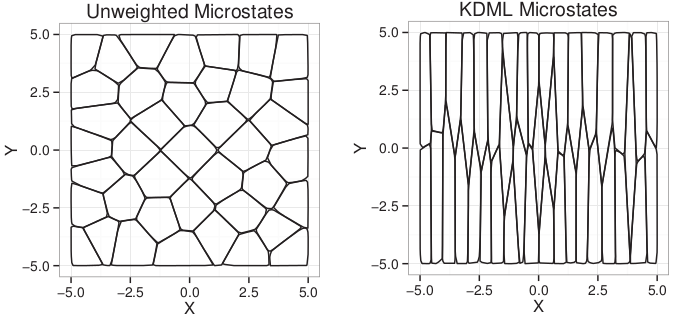
\includegraphics[width=3.2in]{../public/figures/toy_microstates.png}
\caption{Voronoi decomposition of a two dimensional space into forty microstates using both the KDML and unweighted euclidean distance metric with the hybrid K-medoids clustering algorithm.\cite{Beauchamp:2011he} Using KDML, the microstates are geometric elongated in the direction of fast motion and are less likely to contain internal free energy barriers, leading to fewer non-Markovian memory effects without increasing statistical error}
\end{figure}

\begin{figure}
\centering
%\vspace{1em}
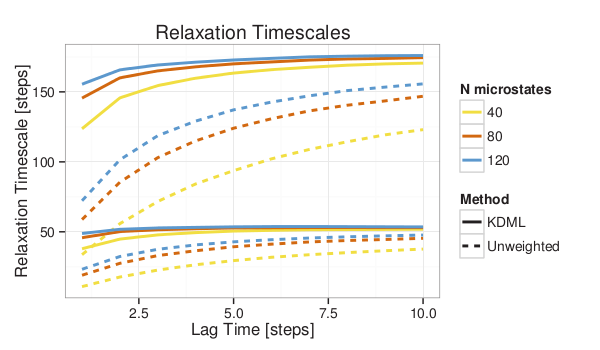
\includegraphics[width=3.2in]{../public/figures/timescales.png}
\caption{Longest two implied timescales for the MSMs produced by different procedures. Dashed curves are for models built using the standard euclidean distance metric, whereas solid lines are for those built using KDML. Models built using KDML are slower and are more Markovian compared to those built using the euclidean metric, even with fewer states.}
\end{figure}

\subsubsection{FiP35 WW}
Next, we apply our approach to a real data set via a reanalysis of two one hundred microsecond simulations of the FiP35 WW domain, performed by D. E. Shaw et al.\cite{Shaw2010}. A previous analysis of this data set using Markov State Model methods revealed the existence of two folding pathways\cite{Lane:2011wj}. However, in order to  achieve a structural resolution in the microstate clustering of greater than $4.5$ \AA, it proved necessary in that study to use more than 26,000 microstates. Parameterizing this model required formally estimating over $6.7 \times 10^8$ pairwise transition probabilities. Because of the obvious potential for overfitting, we ask if it is possible to use KDML to recover more structural and kinetic detail with fewer states.

Comparing models built using the KDML procedure or an unweighted euclidean distance metric, we find two striking results. First, the folding timescale is unchanged by the introduction of the KDML method. In fact, given trends in the estimates of the folding timescale with respect to changes in the number of states (data not shown), we estimate that this analysis significantly underestimates the folding timescale. But more strikingly, our analysis shows the emergence of new discrete timescales in the relaxation spectrum that were not observed with the euclidean distance metrics. While faster than the folding timescale, dynamical processes in the hundreds of nanosecond to microsecond regime are of significant interest. We begin by representing each conformation in the data set by a vector encoding the sine and cosine of its backbone $\Phi$ and $\Psi$ dihedral angles. This has the effect of vectorizing the conformations, as well as breaking the periodic symmetry of the angle measurement. Using these vectors, we apply the KDML procedure with $k=20000$ triplets sampled with $\tau_\mathrm{close}= 2$ ns and $\tau_\mathrm{far}=20$ ns.

\begin{figure}
\centering
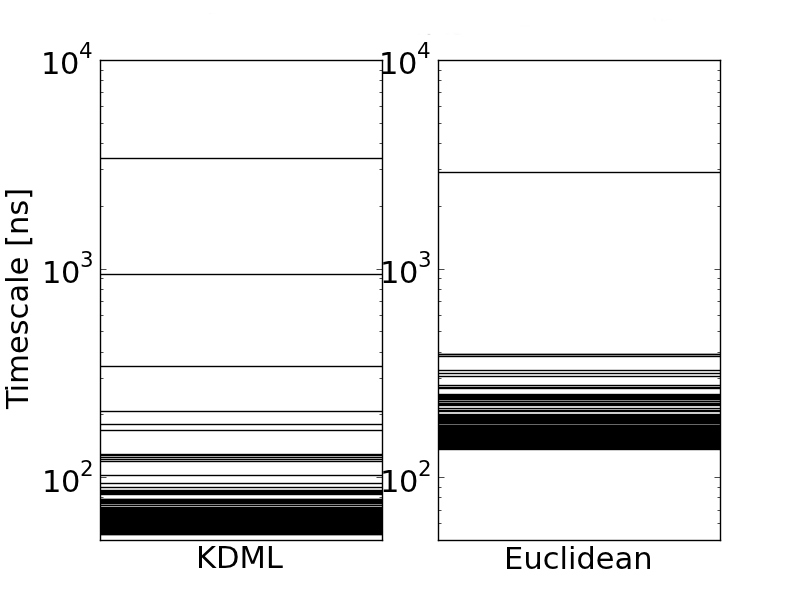
\includegraphics[width=2.5in]{../public/figures/bars.png}

\caption{Two Markov State Models for the FiP35 WW Domain. The model built using the KDML procedure (left) resolves a number of discrete, slow eigenprocesses which were suppressed using the unweighted euclidean distance metric. Both models contain 5000 microstates, a 75 ns lag time, and were built using the same clustering procedure.\cite{Beauchamp:2011he}}
\end{figure}

In order to probe the structural dynamics corresponding to these new timescales, we construct a four macrostate model directly from our five thousand microstate model which seeks to optimally capture the slowest three dynamical processes, using the PCCA+ algorithm.\cite{Deuflhard:2005cp} Visual analysis of the four states reveals that they correspond to the expected folded and unfolded states in addition to two near-native states characterized by rearrangements in the hydrogen bonding structure in the two loop regions. Specifically, one of the states (Fig. 4) shows a reorganization of THR25 forming a nonnative hydrogen bond with HIS23. In the other loop, our final macrostate shows a reorganization of the hydrogen bonding network around ASP15 in which a native hydrogen bond between ASP15 and SER13 is broken and the inflection of the chain at the loop is altered to instead create a set of hydrogen bonds across the loop, including between ARG17O and ARG14N. 

\begin{figure}
\vspace{1em}
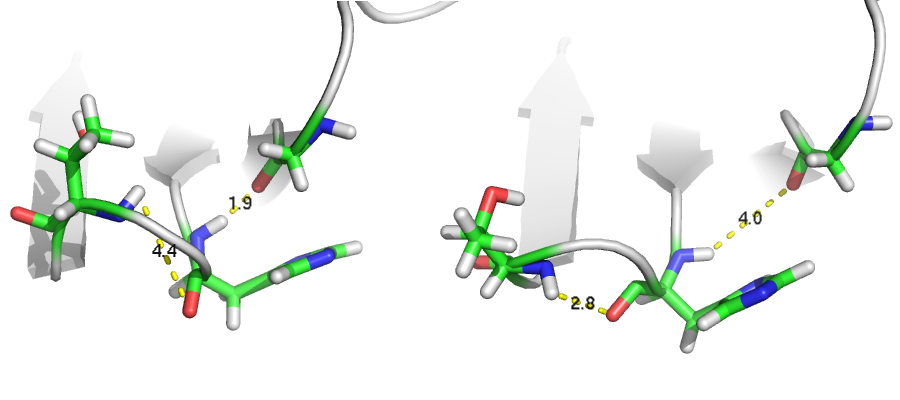
\includegraphics[width=3.2in]{../public/figures/state12.png}
\caption{A representative structure from the simulation's native basin (left) and THR Flip macrostate (right). The subtle structural difference between the two conformational basins, which corresponds to a repacking of the hydrogen bond network in the second hairpin, is identified only via the KDML algorithm.}
\end{figure}

We believe that these discrete metastable but near native states were missed by conventional RMSD based clustering analysis because despite interconverting with the native state slowly, the structural distinctions are subtle. Folding, on the other hand, may be robust to changes in the distance metric because the conformation difference between the folded and unfolded states is so vast. By optimizing the distance metric, we have shown that it is possible to build more accurate Markov state models from finite simulation data. In this work, drawing on recent advances in the machine learning community, we approach that goal within a large-margin Mahalanobis distance metric learning framework.

\section{Future Directions}

\subsection{Statistical Model Selection}
The development of alternative methods of constructing Markov state models, including both the work on KDML (\emph{vide supra}), and time-structure independent components analysis (tICA) which accomplishes a similar goal via correlation function analysis\cite{Schwantes2013Improvements} have brought the issues of model comparison and selection to the fore.
 
In \textcite{Schwantes2013Optimal}, we advocate for the use of likelihood functions, cross validation, and Schwartz's Bayesian Information Criterion (BIC)\cite{Schwartz78Estimating} for MSM model selection. Here, we seek to build models that are \emph{suitably} complex, given the data, yielding complex descriptions of the biomolecular system only to the extent that their additional parameters are implied by the observed dynamics. The central object for model evaluation is now the likelihood function, which given the MSM is expressed as 

\begin{align}
P[x_{0...T-1}] dx^T = \prod_{i=0}^{T-1} T(s(x_i) \rightarrow s(x_{i+1})) \cdot \prod_{i=0}^{T} p_{s(x_i)}(x_{i})
\label{eq:like}
\end{align}

\begin{equation}
\label{eq:bic}
\mathrm{BIC} \equiv -2\cdot \ln L + k \cdot \ln N
\end{equation}

The challenging portion of this computation is the so-called emission model -- using the language of the hidden Markov model (HMM) literature\cite{Rabiner1986Introduction} -- $\prod_{i=0}^{T} p_{s(x_i)}(x_{i}))$. For the standard MSM whose states are a Voronoi tessellation over phase space, $p_{s(x_i)}(x_i) \, dx_i$ is naturally the probability density of a uniform distribution over the volume of the state, whose normalization requires the computation of the volumes of the states. While trivial in two or three dimensions, this computational geometry task becomes challenging in high-dimensional settings. The computation of such volumes has occupied significant attention in recent years in the computational geometry literature, especially via randomized algorithms\cite{Kannan97, Simonovits03, Lovasz03}. In this work, we opt to approximate the volumes using na\"{i}ve Monte Carlo rejection sampling, which we find tractable for large systems only when the molecular dynamics data set is first projected into a suitable small vector space of up to perhaps ten dimensions.

Nonetheless, we hope to show that the use of likelihood functions over the trajectories though \emph{phase space}, as opposed to their likelihood through simply the projected state space, is critical for correct selection and opens the door to a vast set of statistical model selection tools.

\subsection{MSM--Accelerated Molecular Dynamics}
For a number of years, it has been clear that Markov state models provide a framework for running simulations more efficiently, avoiding wasted-effort sampling areas of phase space that have already been exhaustively explored while other regions remain undiscovered\cite{Bowman2010Enhanced, Weber2011Characterization}.

I am currently leading the development of an implementation of this procedure, called MSMAccelerator in modern, extensible, distributed python environment. MSMAccelerator combines two existing technologies: OpenMM for GPU-accelerated molecular simulations\cite{Eastman2013OpenMM} and MSMBuilder for the construction of stochastic network models \cite{Beauchamp:2011he}. We hope to provide this package as a widely available, GPL-licensed platform that makes improvements simulation protocols and MSM construction available to the widest possible audience.

In collaboration with G. Kiss and M. P. Harrigan, we are using MSMAcclerator to simulate three systems: dynamics on the two-dimensional M\"{u}ller potential, the folding of the ultrafast-folding norleucine mutant of the HP35 Villin headpiece domain\cite{Kubelka2006Sub}, and conformation change dynamics in HIV-1 protease. Early indications are that MSM methods may enable a ~10$\times$ speed up in conformational sampling.

\subsection{A Markov-Switching Autoregressive Model}

One of the deficiencies of current-generation MSMs is their treatment of within-state dynamics, which are assumed to be infinitely fast with respect to the Markov lag time. In practice, satisfying this assumption requires increasing the lag time -- in protein folding data sets lag times of ~ 50 ns are common -- in such a way that we significantly sacrifice temporal resolution. The balance between the desire for model resolution and model accuracy is subtle here: by simply taking the lag-time to be longer than the system's longest relaxation timescale, we could have a ``perfect'' model based on likelihood criterion that features one-step equilibration.

I am currently developing a new family of models for protein dynamics called Markov-switching autoregressive models (MSArMs) that generalize both standard MSMs and stable stochastic diffusion models (\emph{i.e.} discrete-time Ornstein-Uhlenbeck processes). Such models have been used in the econometrics literature, and were originally introduced by Hamilton\cite{Hamilton1989New, Hamilton1990Analysis} to study fluctuations in United States gross national product (GNP), subject to latent Markov dynamics between two economic regimes, those of normal growth and recession.

As alluded to above, the two components of the model are a discrete-time Ornstein-Uhlenbeck process, also known as an AR(1) model in the econometrics literature, and a latent discrete-state Markov chain. The diffusion process evolves according to

\begin{align}
X_t = \mathbf{A}_{s_t} (X_{t-1} - \mu_{s_t}) + \mathcal{N}(\mu_{s_t}, \mathbf{\Sigma}_{s_t})
\end{align}

which corresponds physically to Langevin dynamics of a thermalized harmonic oscillator in the highly overdamped regime. The parameters of the oscillator ($\mathbf{A}$, $\mu$, $\Sigma$ which are interpretable as a friction coefficient, mean position and force constant) jump around via a discrete-state Markov chain.

\begin{align}
P(s_t = j | s_{t-1} = i) = T_{ij}
\end{align}

In this model, the fast within-state dynamics are described effectively by the equivalent of a friction coefficient. The within-state correlation timescales are given by $-1/\ln \lambda$ where $\lambda$ are the eigenvalues of $\mathbf{A}$, which correspond to the fast manifold of the transfer operator\cite{Prinz2011Markov}, while the slow dynamics are described by the Markov jump process.

While still young, I am hopeful that this model will remedy a major deficiency in current MSM methodologies by providing a first-order description of the within-state dynamics, relaxing the assumption that such dynamics are described by i.i.d. samples from a state's distribution at every time step, permitting much higher spatial and temporal resolution by using a model better suited to the physics of the generating process.

\section{Conclusions}

In my view, the field of statistical modeling of protein conformational dynamics, driven by the exponential increase in the amount of available simulation data, is a very young and fruitful field. We can simply do things today that would have been impossible as little as five years ago. I anticipate that over the course of my Ph.D. I will be able to make substantial contributions to its development.


\bibliography{bibliography}
\end{document}
